\subsubsection{AlexNet}
%
AlexNet is a famous \acrshort{cnn} which was developed in 2012 by \textcite{krizhevsky_imagenet_2012}. It was a breakthrough in the deep \acrshort{cnn} field and this model won the ImageNet competition. Krizhevsky et al. used some parameter optimizations and made the model deeper to considerably improve the learning ability of the CNN \cite{khan_survey_2020}. It is composed of 5 convolutional layers and 3 fully-connected layers, as seen in Figure \ref{fig:alexnet}. Each convolutional layer has a ReLU activation function and it uses pooling.
%
\begin{figure}[H]
    \centering
    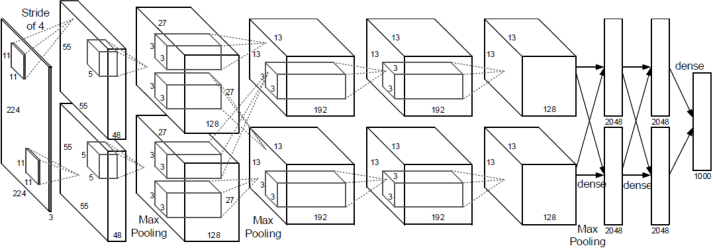
\includegraphics[width=\textwidth]{alexnet.pdf}
    \caption{An illustration of the architecture of AlexNet, from \cite{krizhevsky_imagenet_2012}}
    \label{fig:alexnet}
\end{figure}
%
\subsubsection{VGG}
%
After the success of AlexNet in 2012, research was carried out to reduce the computational complexity while keeping accuracy. In 2014, VGG, a deeper variant of AlexNet was developed by \textcite{simonyan_very_2015}. It is composed of 5 groups of convolutional layers, where the number of layers depends on the version of VGG. It won the localization in the ImageNet challenge in 2014 \cite{simonyan_very_2015}. An illustration is provided in Figure \ref{fig:vgg}. This level of depth was possible thanks to the application of very small ($3 \times 3$) convolution kernels. They allow a larger receptive field with fewer parameters and more non-linearities than a larger kernel \cite{matteucci_artificial_2019}. However, it has a high memory request. 100MB per image needs to be stored in all \acrshort{fm}s for the forward propagation \cite{matteucci_artificial_2019}.
%
\begin{figure}[H]
    \centering
    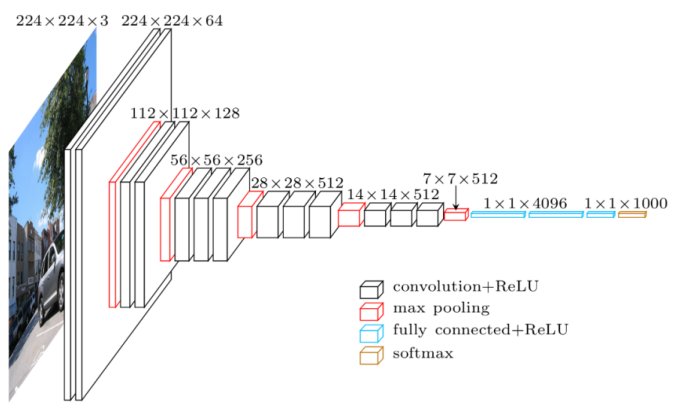
\includegraphics[width=0.75\textwidth]{VGG.pdf}
    \caption{An illustration of the architecture of VGG16, from \cite{simonyan_very_2015}}
    \label{fig:vgg}
\end{figure}
%
\subsubsection{ResNet}
%
\textcite{he_deep_2016} developed ResNet in 2015. It is a very deep network which can contain from 50 to 1000 convolutional layers. It is composed of structures that are more complex and irregular than in the networks described previously. \textcite{he_deep_2016} showed that an increase in the depth of the network does not lead to an improvement in the performance. Indeed, beyond a certain amount of layers, a continuous increase of the depth leads to the degradation of the accuracy. This is not due to overfitting. It is because the deeper models are harder to optimize than shallower ones (vanishing gradient described in Section \ref{subs:trainbackward}) \cite{matteucci_artificial_2019}. 

However, deeper networks should at least have similar or better performance than shallower ones. Indeed, let’s compare a deep and a shallow network. If the deeper network is composed of the same layers than the shallower one and that the other added layers are just identity mapping, then the network should have the same performance as the shallower one. Therefore, a deeper network should not have worse performance than shallower ones \cite{matteucci_artificial_2019}.

To overcome this issue, \textcite{he_deep_2016} introduced an \textit{identity shortcut connection} which skips one or more layers and set weights to the identity, as can be seen in Figure \ref{fig:resnet}. These weights associated with the shortcut connection can be used to learn a residual $\mathcal{F}(x)$ to improve the solution. The performance of this very deep network allowed it to win the 2015 ILSVR for both localization and classification.
%
\begin{figure}[H]
    \centering
    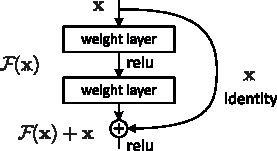
\includegraphics[width=0.7\textwidth]{resnet.pdf}
    \caption{ResNet building block, from \cite{he_deep_2016}}
    \label{fig:resnet}
\end{figure}
%
\subsubsection{MobileNetV2} \label{subs:mbv2}
%
According to \textcite{cheng_recent_2018}, the performance of \acrshort{cnn} in recent years became outstanding. These improvements came at the cost of storage and computational complexity. It is not an issue for the \acrshort{cnn} training phase, because the GPU and CPU also gained in computational units and memory. However, for the inference phase, the computational complexity and the storage requirements are way beyond the capabilities of most of the embedded applications and mobile devices such as \acrshort{fpga} \cite{cheng_recent_2018}.
%
\begin{itemize}
    \item The enormous computational complexity of \acrshort{cnn}s makes it difficult to deploy on real-time applications and it consumes battery power.
    \item The large number of parameters of \acrshort{cnn}s consumes considerable storage and run-time memory.
\end{itemize}

To overcome this issue, \textcite{sandler_mobilenetv2_2018} introduced a network called MobileNetV2 in 2018. It is specifically developed for constrained environments. First, the size and number of operations are decreased thanks to DSC (see Section \ref{subs:dsc}) and thanks to a new type of layer \textit{inverted residual with a linear bottleneck} that performs the bottleneck convolution, which can be observed in Figure \ref{fig:invreslinbot} and Table \ref{tab:invreslinbot}.
This layer is composed of a $1 \times 1$ convolution to expand the number of the input \acrshort{fm} channels by a factor $t$ ($N_{intf} = t \times N_{if}$). It is then followed by a \acrshort{dsc}. The purpose of the first convolution layer which increases the number of channels is supposed to counterbalance the loss of information that occurred by the ReLU activation. They also added a skip connection to build a network of great depth, and the last convolution has a linear activation function \cite{sandler_mobilenetv2_2018}.

%
\begin{figure}[H]
    \centering
    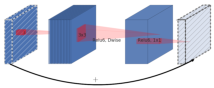
\includegraphics[width=\textwidth]{mbnv2.pdf}
    \caption{inverted residual with linear bottleneck, from \cite{sandler_mobilenetv2_2018}}
    \label{fig:invreslinbot}
\end{figure}

\begin{table}
    \center
    \begin{tabular}{c|c|c}
        Input & Operator & Output \\
        \hline \hline
        $N_{ix} \times N_{iy} \times N_{if}$ & $1 \times 1$ conv2d, ReLU6 & $N_{ix} \times N_{iy} \times (t \times N_{if})$ \\
        $N_{ix} \times N_{iy} \times (t \times N_{if})$ & $3 \times3$ dwise s=$s$, ReLU6 & $\frac{N_{ix}}{s} \times \frac{N_{iy}}{s} \times (t \times N_{if})$ \\
        $\frac{N_{ix}}{s} \times \frac{N_{iy}}{s} \times (t \times N_{if})$ & $1 \times 1$ conv2d & $\frac{N_{ix}}{s} \times \frac{N_{iy}}{s} \times N_{of}$ \\
        \hline \hline
    \end{tabular}
    \caption{Bottleneck convolution, from \cite{sandler_mobilenetv2_2018}}
    \label{tab:invreslinbot}
\end{table}

MobileNetV2 is also composed of standard convolution, pooling, and $1 \times 1$ convolution layers. More information about the structure of MobileNetV2 can be found in Appendix \ref{appendix:mbv2}. In the frame of this thesis, we design an \acrshort{fpga}-based accelerator that implements MobileNetV2.
